\section{Checking model conditions using graphs}

%%%%%%%%%%%%%%%%%%%%%%%%%%%%%%%%%%%%

\begin{frame}
\frametitle{Modeling conditions}

\[ \hat{y} = \beta_0 + \beta_1 x_1 + \beta_2 x_2 + \cdots + \beta_p x_p \] 

$\:$ \\

The model depends on the following conditions
\begin{enumerate}
\item residuals are nearly normal (primary concern relates to residuals that are outliers)
\item residuals have constant variability
\item residuals are independent
\item each variable is linearly related to the outcome \\
\end{enumerate}

We often use graphical methods to check the validity of these conditions, which we will go through in detail in the following slides.

\end{frame}

%%%%%%%%%%%%%%%%%%%%%%%%%%%%%%%%%%

\begin{frame}
\frametitle{(1) nearly normal residuals}

normal probability plot and/or histogram of residuals: \\

\begin{center}
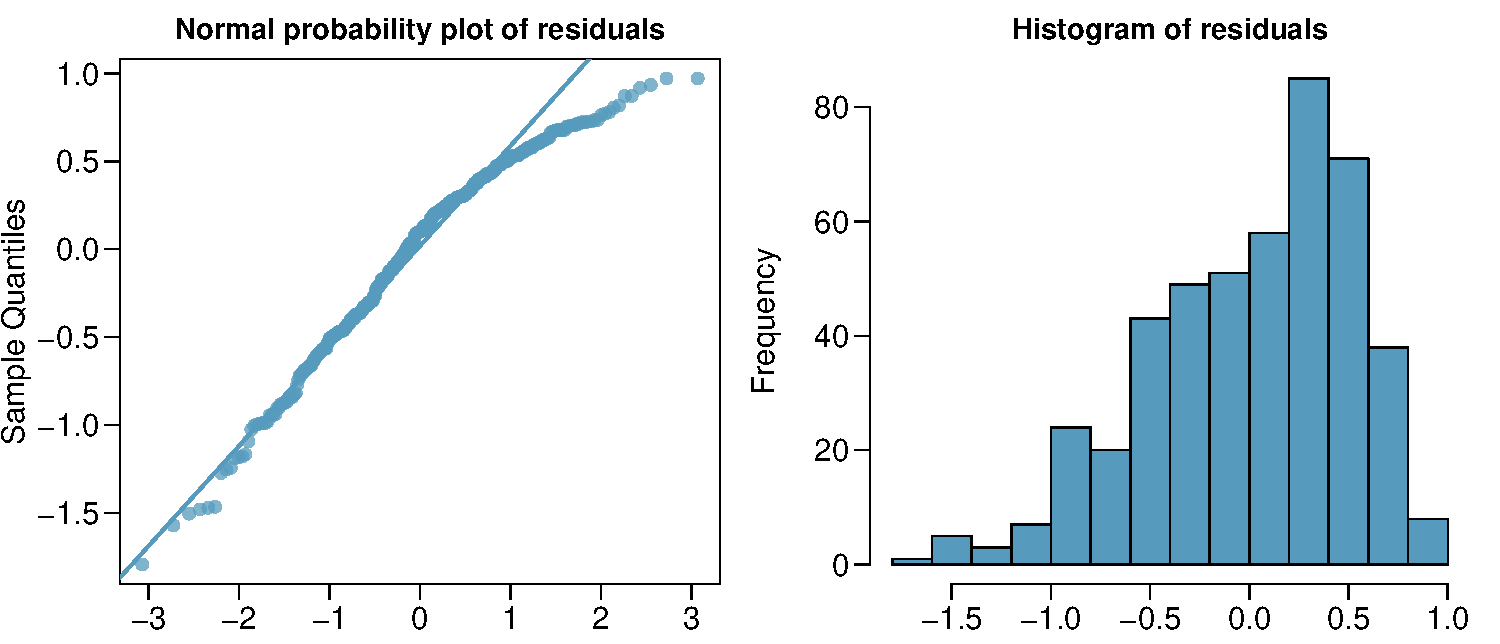
\includegraphics[width=\textwidth]{8-3_model_cond/figures/beauty/normal_res}
\end{center}

\dq{Does this condition appear to be satisfied?}

\end{frame}

%%%%%%%%%%%%%%%%%%%%%%%%%%%%%%%%%%

\begin{frame}
\frametitle{(2) constant variability in residuals}

scatterplot of residuals and/or absolute value of residuals vs. fitted (predicted): \\

\begin{center}
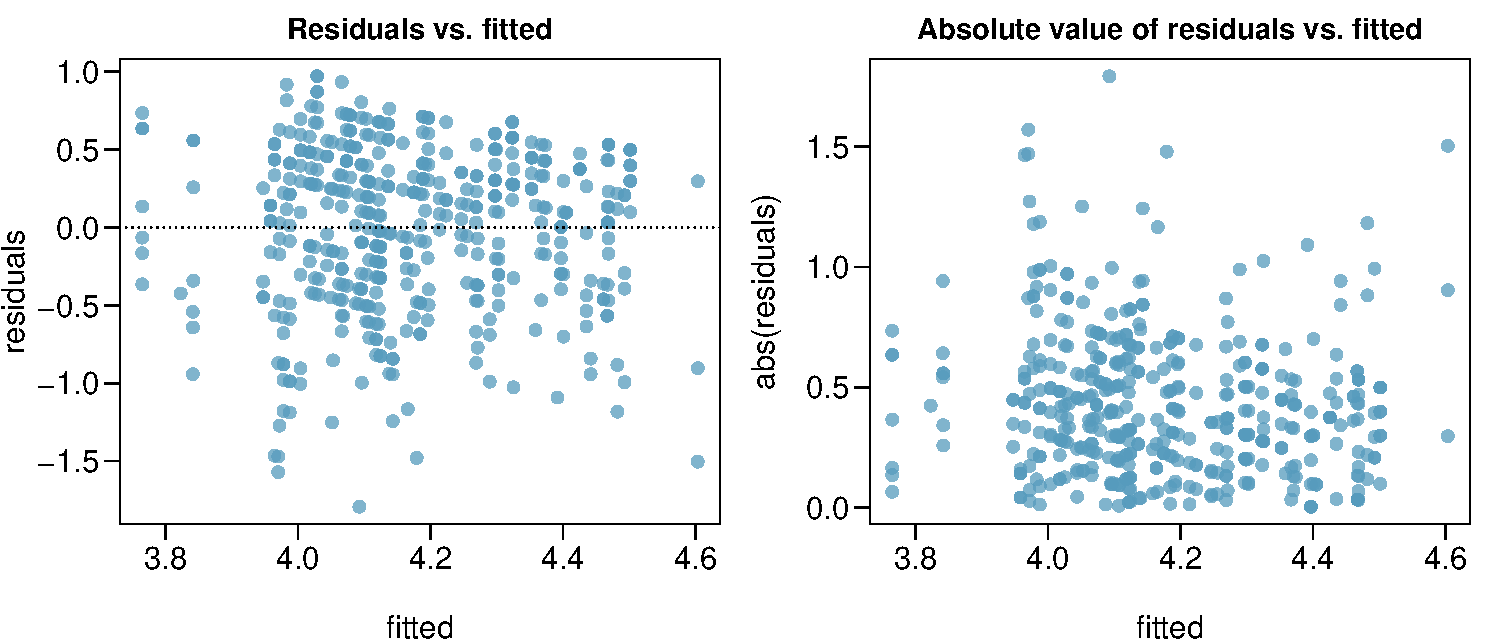
\includegraphics[width=\textwidth]{8-3_model_cond/figures/beauty/homo_res}
\end{center}

\dq{Does this condition appear to be satisfied?}

\end{frame}

%%%%%%%%%%%%%%%%%%%%%%%%%%%%%%%%%%

\begin{frame}
\frametitle{Checking constant variance - recap}

\begin{itemize}

\item When we did simple linear regression (one explanatory variable) we checked the constant variance condition using a plot of \hl{residuals vs. x}.

\item With multiple linear regression (2+ explanatory variables) we checked the constant variance condition using a plot of \hl{residuals vs. fitted}. 

\end{itemize}

$\:$ \\

\dq{Why are we using different plots?}

\soln{\only<2>{In multiple linear regression there are many explanatory variables, so a plot of residuals vs. one of them wouldn't give us the complete picture.
}}

\end{frame}

%%%%%%%%%%%%%%%%%%%%%%%%%%%%%%%%%%

\begin{frame}[fragile]
\frametitle{(3) independent residuals}

scatterplot of residuals vs. order of data collection: \\

\begin{center}
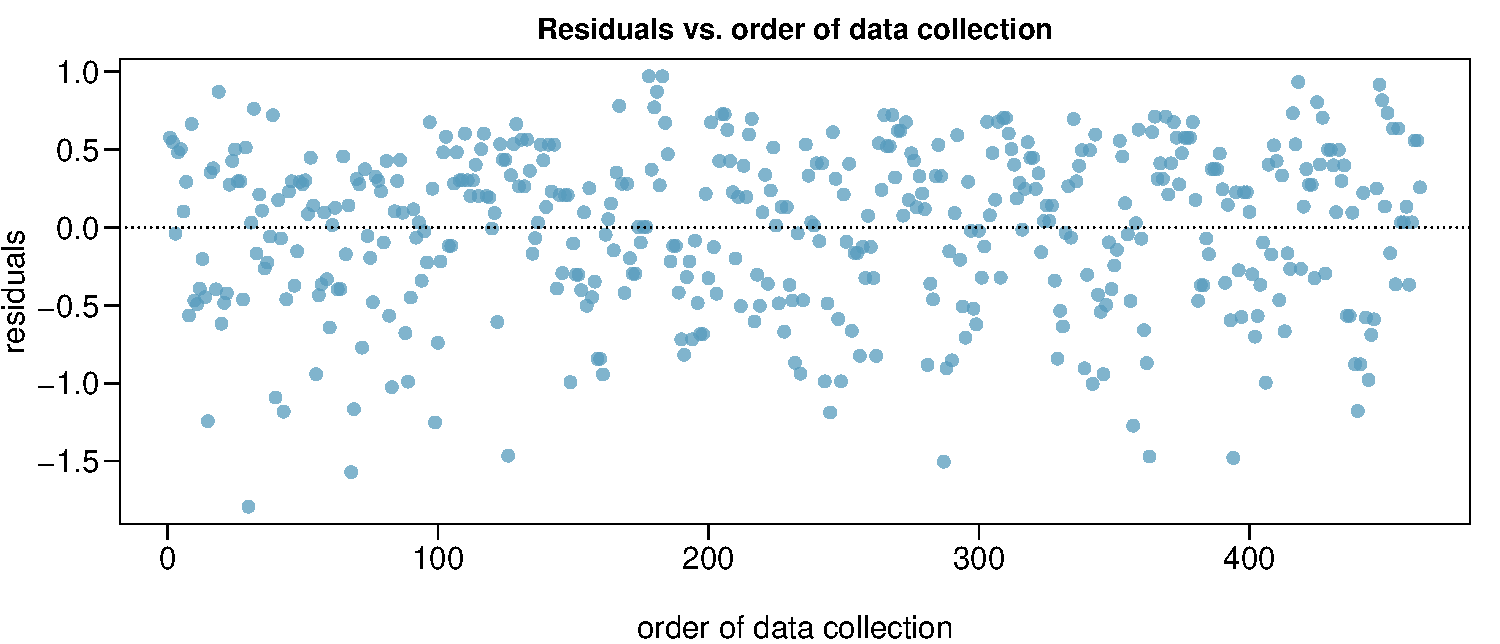
\includegraphics[width=0.8\textwidth]{8-3_model_cond/figures/beauty/indep_res}
\end{center}

\dq{Does this condition appear to be satisfied?}

\end{frame}

%%%%%%%%%%%%%%%%%%%%%%%%%%%%%%%%%%

\begin{frame}
\frametitle{More on the condition of independent residuals}

\begin{itemize}

\item Checking for independent residuals allows us to indirectly check for independent observations.

\item If observations and residuals are independent, we would not expect to see an increasing or decreasing trend in the scatterplot of residuals vs. order of data collection.

\item This condition is often violated when we have time series data. Such data require more advanced time series regression techniques for proper analysis.

\end{itemize}

\end{frame}

%%%%%%%%%%%%%%%%%%%%%%%%%%%%%%%%%%

\begin{frame}[fragile]
\frametitle{(4) linear relationships}

scatterplot of residuals vs. each (numerical) explanatory variable:

\begin{center}
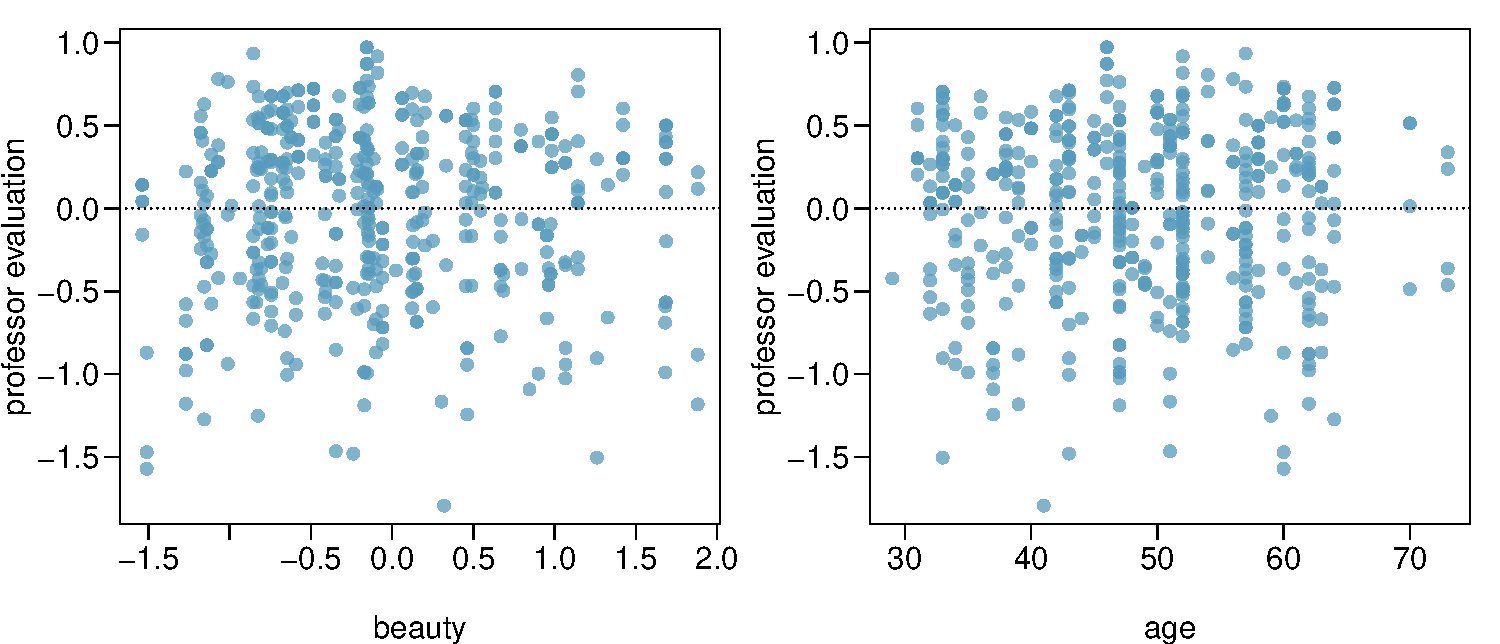
\includegraphics[width=0.8\textwidth]{8-3_model_cond/figures/beauty/linear}
\end{center}

\dq{Does this condition appear to be satisfied?}

\Note{We use residuals instead of the predictors on the y-axis so that we can still check for linearity without worrying about other possible violations like collinearity between the predictors.}

\end{frame}

%%%%%%%%%%%%%%%%%%%%%%%%%%%%%%%%%%%